\documentclass[conference]{IEEEtran}
\usepackage{times}

% numbers option provides compact numerical references in the text. 
\usepackage[numbers]{natbib}
\usepackage{multicol}
\usepackage[bookmarks=true]{hyperref}
\usepackage{amsmath,amssymb}
\usepackage{amsthm}
\usepackage{mathtools}
\usepackage{graphicx}
% \usepackage{caption}
\usepackage{float}
\usepackage{subcaption}
\usepackage{epstopdf}
% \usepackage{subfig}
\usepackage{algorithm}
\usepackage[noend]{algpseudocode}
\makeatletter
\def\BState{\State\hskip-\ALG@thistlm}
\makeatother

\usepackage{tabstackengine}
\stackMath

\usepackage{tikz}
\usetikzlibrary{scopes}
\usetikzlibrary{shapes.misc}
\tikzset{cross/.style={cross out, draw=black, minimum size=2*(#1-\pgflinewidth), inner sep=0pt, outer sep=0pt},
%default radius will be 1pt.
cross/.default={2pt}}

\newtheorem{theorem}{Theorem}
\newtheorem{proposition}{Proposition}
\newcommand\numberthis{\addtocounter{equation}{1}\tag{\theequation}}
\DeclareMathOperator{\sign}{\text{sgn}}
\DeclareMathOperator*{\argmin}{arg\,min}
\DeclareMathOperator{\intr}{int}
\DeclareMathOperator{\dom}{dom}

\newcommand{\EH}[1]{{\color{blue} {Eric: {#1}}  }}

\pdfinfo{
   /Author (Eric Huang)
   /Title  (Robots: Our new overlords)
   /CreationDate (D:20161016120000)
   /Subject (Robots)
   /Keywords (Robots;Overlords)
}

\begin{document}

% paper title
\title{Robotic Pulling}

% You will get a Paper-ID when submitting a pdf file to the conference system
% \author{Author Names Omitted for Anonymous Review. Paper-ID [add your ID here]}

%\author{\authorblockN{Michael Shell}
%\authorblockA{School of Electrical and\\Computer Engineering\\
%Georgia Institute of Technology\\
%Atlanta, Georgia 30332--0250\\
%Email: mshell@ece.gatech.edu}
%\and
%\authorblockN{Homer Simpson}
%\authorblockA{Twentieth Century Fox\\
%Springfield, USA\\
%Email: homer@thesimpsons.com}
%\and
%\authorblockN{James Kirk\\ and Montgomery Scott}
%\authorblockA{Starfleet Academy\\
%San Francisco, California 96678-2391\\
%Telephone: (800) 555--1212\\
%Fax: (888) 555--1212}}


% avoiding spaces at the end of the author lines is not a problem with
% conference papers because we don't use \thanks or \IEEEmembership


% for over three affiliations, or if they all won't fit within the width
% of the page, use this alternative format:
% 
%\author{\authorblockN{Michael Shell\authorrefmark{1},
%Homer Simpson\authorrefmark{2},
%James Kirk\authorrefmark{3}, 
%Montgomery Scott\authorrefmark{3} and
%Eldon Tyrell\authorrefmark{4}}
%\authorblockA{\authorrefmark{1}School of Electrical and Computer Engineering\\
%Georgia Institute of Technology,
%Atlanta, Georgia 30332--0250\\ Email: mshell@ece.gatech.edu}
%\authorblockA{\authorrefmark{2}Twentieth Century Fox, Springfield, USA\\
%Email: homer@thesimpsons.com}
%\authorblockA{\authorrefmark{3}Starfleet Academy, San Francisco, California 96678-2391\\
%Telephone: (800) 555--1212, Fax: (888) 555--1212}
%\authorblockA{\authorrefmark{4}Tyrell Inc., 123 Replicant Street, Los Angeles, California 90210--4321}}


\maketitle

\begin{abstract}
\end{abstract}

\IEEEpeerreviewmaketitle

\section{Introduction}

\section{Theory}

\subsection{Planar Pulling Subject to Friction}

We present a preliminary quasi-static analysis of planar pulling
subject to friction. Planar pulling is the manipulation skill where
the robot contacts a rigid body at a point and pulls that contact
point along a trajectory. 

Let the \textit{generalized velocity} of a planar rigid body be
$\mathbf{v}^+ = [v_x, v_y, \omega]^T$, where $v_x$ and $v_y$ are the
linear velocities of a reference point and $\omega$ is the angular
velocity about that point. Taking the origin as the reference point,
the velocity of a point $\mathbf{x}$ on the body is then given by
$\mathbf{v}(\mathbf{x}) = [v_x, v_y]^T + \omega\hat{\mathbf{k}} \times
\mathbf{x}$ and can be written in matrix notation as
\begin{equation} \label{eq:generalized-velocity}
\mathbf{v}(\mathbf{x}) = A(\mathbf{x})\mathbf{v}^+,
\end{equation}
where
\begin{equation}
  A(\mathbf{x}) = 
  \begin{bmatrix*}[r]
    1 & 0 & -x_2 \\
    0 & 1 &  x_1
  \end{bmatrix*}.
\end{equation}

In this analysis, we choose a coordinate frame such that the origin is
the contact point and the $y$-axis aligns with the contact point
velocity (see Figure \ref{fig:presspull-motion} for an example). Then
the total frictional force and moment of the body at the origin are
\begin{align}
  % Force
  % \mathbf{f}_f &= -\mu\,\sign(\dot{\theta})\,\mathbf{\hat{k}}\,\times\int_{R}\frac{\mathbf{r}-\mathbf{r_{\text{IC}}}}{\lVert \mathbf{r}-\mathbf{r_{\text{IC}}} \rVert} p(\mathbf{r}) dA \\
  % \mathbf{f}_f &= -\mu\int_{R}\frac{A(\mathbf{r})\mathbf{v}^+}{\lVert A(\mathbf{r})\mathbf{v}^+ \rVert} p(\mathbf{r}) dA \\
  \mathbf{f}_f &= -\mu\int_{R}\frac{\mathbf{v}(\mathbf{r})}{\lVert \mathbf{v}(\mathbf{r}) \rVert} p(\mathbf{r}) dA \\
  % Moment
  % \mathbf{m}_f &= -\mu\,\sign(\dot{\theta}) \int_{R}\mathbf{r}\cdot\frac{\mathbf{r}-\mathbf{r_{\text{IC}}}}{\lVert \mathbf{r}-\mathbf{r_{\text{IC}}} \rVert} p(\mathbf{r}) dA,
  % \mathbf{m}_f &= -\mu\int_{R}\mathbf{r}\times\frac{A(\mathbf{r})\mathbf{v}^+}{\lVert A(\mathbf{r})\mathbf{v}^+ \rVert} p(\mathbf{r}) dA,
  \mathbf{m}_f &= -\mu\int_{R}\mathbf{r}\times\frac{\mathbf{v}(\mathbf{r})}{\lVert \mathbf{v}(\mathbf{r}) \rVert} p(\mathbf{r}) dA,
\end{align}
where $\mu$ is the coefficient of friction, $R$ is the region of the
rigid body in contact with the plane, $\mathbf{v}(\mathbf{r})$ is the
body point velocity given by (\ref{eq:generalized-velocity}) and
$p(\mathbf{r})$ is a pressure distribution over $R$.
\begin{equation}
\begin{aligned}
& \underset{\mathbf{v}^+}{\text{minimize}}
& & \mu\int_R\lVert A(\mathbf{r})\mathbf{v}^+ \rVert p(\mathbf{r}) dA \\
& \text{subject to}
& & \mathbf{v}^+ \in \mathcal{C} 
\end{aligned} \label{eq:constrained-frictional-dissipation}
\end{equation}
Without loss of generality, we take
$\mathcal{C} = \{[0,1,\omega]^T, \omega \in \mathbb{R}\}$ so that the
contact point motion is aligned with the coordinate frame. We call the
objective in (\ref{eq:constrained-frictional-dissipation}) the
frictional dissipation equation $\mathrm{P}(\mathbf{v}^+)$.



\begin{equation} \label{eq:frictional-dissipation}
  \mathrm{P}(\mathbf{v}^+) = \mu\int_R\lVert \mathbf{v}(\mathbf{r}) \rVert p(\mathbf{r}) dA
\end{equation}
Form the Lagrangian
\begin{equation}
  \mathrm{L}(\mathbf{v}^+,\mathbf{\lambda}) = \mathrm{P}(\mathbf{v}^+) - \lambda_1(v^+_1 - 1) - \lambda_2v^+_2
\end{equation}
The gradient of $\mathrm{L}$ with respect to $\mathbf{v}^+$ is
\begin{equation}
  \nabla\mathrm{L}(\mathbf{v}^+,\mathbf{\lambda}) = \mu\int_R\frac{A(\mathbf{r})^TA(\mathbf{r})\mathbf{v}^+}{\lVert A(\mathbf{r})\mathbf{v}^+ \rVert} p(\mathbf{r}) dA - \begin{bmatrix}\lambda_1, \lambda_2, 0\end{bmatrix}^T
\end{equation}
After some work, we end up with the following conditions on the force and the moment
\begin{align}
  \mathbf{f}_f &= -\begin{bmatrix}\lambda_1, \lambda_2\end{bmatrix}^T\\
  \mathbf{m}_f &= 0
\end{align}

We prefer the minimum power interpretation in our theoretical analysis
for a few reasons. For bodies with discrete points of support, the
minimum still exists whereas the moment may be indeterminate.

% \begin{enumerate}
% \item Pull contact setup
% \item Generalized velocities
% \item A(x)
% \item Dissipation function (convex)
% \item Pressure distribution p(r)
% \item Lagrangian of pulling
% \item Force balance
% \item Moment balance
% \item Discrete pressure distributions
% \end{enumerate}

\subsection{Quasi-static Stability}

% Press-pull stability theorem figure.
\begin{figure}
  \centering
  \def\iangle{35} % Angle of the inclined plane
  \begin{tikzpicture}[
    scale=1.25, every node/.style={scale=1.25},
    force/.style={>=latex,draw=black,fill=black},
    axis/.style={densely dashed,draw=gray,font=\small},
    ]
    \fill[draw=black,fill=blue!10,thin,rotate=\iangle] (-0.3,-0.5) rectangle (2.3,.5);
    \draw[rotate=\iangle] (1,0) circle[radius=2.4pt] node[cross] {};
    \draw[rotate=\iangle] (1,0) node[above right] {\tiny CoP};
    {[axis,->]
      \draw (0,0) -- (2.5,0) node[right] {$x$};
      \draw (0,0) -- (0,2.5) node[above] {$y$};
    }
    {[force,->]
      \draw (0,0) -- ++(0,1.5) node[right] {$\mathbf{v}_c$};
    }
    \fill (0,0) circle [radius=1.pt];
    \fill (1.2207,0) circle [radius=1.pt] node[below right] {$x_{\text{\tiny IC}}$};
  \end{tikzpicture}
  \caption{Motion of a press-pulled slider.}
  \label{fig:presspull-motion}
\end{figure}

\begin{theorem}
  For pulling of a rigid body in the plane, the line from the pulling
  contact point to the body's center of pressure converges to the line
  of motion.
\end{theorem}

\begin{proof}
  % TODO Shorten this proof. Rewrite to use generalized velocities.
  Let the $y$-axis of the coordinate frame be aligned with the line of
  motion of the press-pull contact point (see Figure
  \ref{fig:presspull-motion} for an example). Then the instantaneous
  rotation center of the body must fall on the $x$-axis, and we can
  write $\mathbf{r}_\text{IC} = (x_\text{IC},0)^T$.

  Suppose the center of pressure is strictly to the right of the line
  of motion (as in Figure \ref{fig:presspull-motion}). Then by Theorem
  7.4 in \cite{Mason}, the rotation center lies on the positive
  $x$-axis and has negative rotation. The velocity of a point on the
  rigid body is given by
  $\mathbf{v}(\mathbf{r}) =
  \dot{\theta}\,\hat{\mathbf{k}}\times(\mathbf{r} -
  \mathbf{r}_\text{IC})$.
  We can compute the motion of the body relative to the contact point
  by
  \begin{align*}
    \mathbf{v}(\mathbf{r}) - \mathbf{v}_c &= \dot{\theta}\,\hat{\mathbf{k}}\times(\mathbf{r} - \mathbf{r}_\text{IC}) - \dot{\theta}\,\hat{\mathbf{k}}\times(\mathbf{0} - \mathbf{r}_\text{IC}) \\
    &= \dot{\theta}\,\hat{\mathbf{k}}\times(\mathbf{r} - \mathbf{0}) \numberthis \label{eqn:rel-rotation-center},
  \end{align*}
  where $\mathbf{v}_c$ is the velocity of the contact point. In other
  words, the body is rotating clockwise relative to the
  contact point with angular velocity
  \begin{equation}
    \dot{\theta} = -\frac{\lVert\mathbf{v}_c\rVert}{x_\text{IC}}.
  \end{equation}

  Let $\theta \in (\pi/2, -\pi/2)$ be the orientation of the center of
  pressure in the frame of the contact point. When the line of motion
  passes through the center of pressure, a pure translation takes
  place (Theorem 7.4 in \cite{Mason}). This implies that
  $\dot{\theta} = 0$ if and only if $\theta = \pi/2, -\pi/2$. Since
  $\theta$ is monotonically decreasing, we see that it must converge
  to $-\pi/2$ in the limit as $t \rightarrow \infty$.

  The case when the center of pressure is strictly to the left of the
  line of motion follows from symmetry about the $y$-axis.
\end{proof}

Note that the above proof holds for \textit{all pressure
  distributions} of the body on the support
surface.

% \begin{proposition}
%   When pressing down on a point contact on a rigid body, the center of
%   pressure is given by
%   \begin{equation}
%     \text{CoP} = \frac{1}{f_0 + p_c}\left(\int_R\mathbf{r}p(\mathbf{r})dA + \mathbf{r}_cp_c\right)
%   \end{equation}
% \end{proposition}
% In other words, the resulting center of pressure is located on the
% line segment between the contact point and the original center of
% pressure. 

% \begin{proposition}
%   A rigid body in the plane can be moved from A to B with arbitrary
%   accuracy using at most two press-pulls.
% \end{proposition}

\subsection{Frictional Force \& Moment Envelopes}

\begin{figure*}[ht]
  \centering
  \begin{subfigure}[b]{0.24\textwidth}
    \centering
    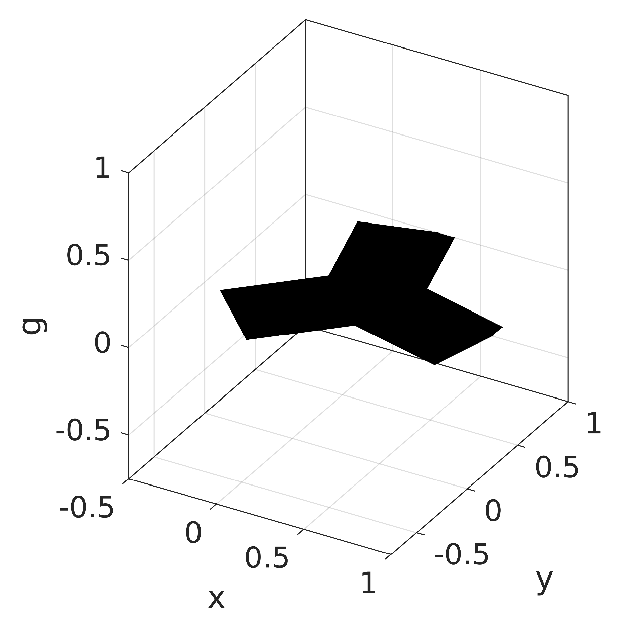
\includegraphics[width=1\linewidth]{./fig/moment_hull_1}
    \caption{}
  \end{subfigure}
  \begin{subfigure}[b]{0.24\textwidth}
    \centering
    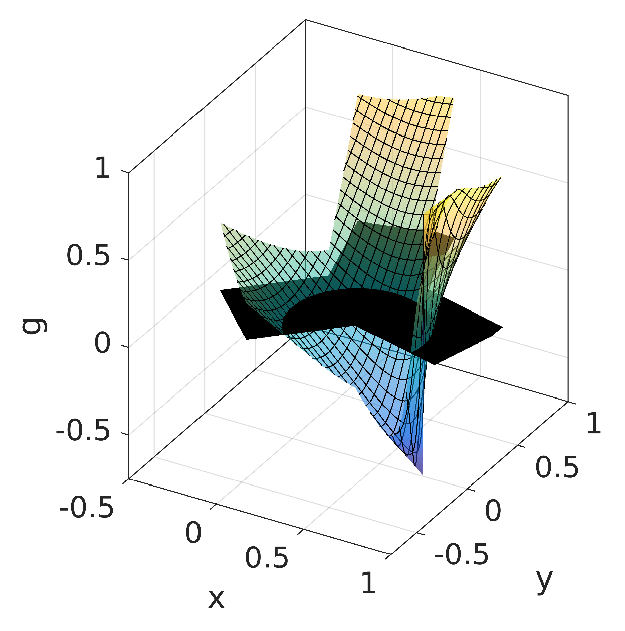
\includegraphics[width=1\linewidth]{fig/moment_hull_2}
    \caption{}
  \end{subfigure}
  \begin{subfigure}[b]{0.24\textwidth}
    \centering
    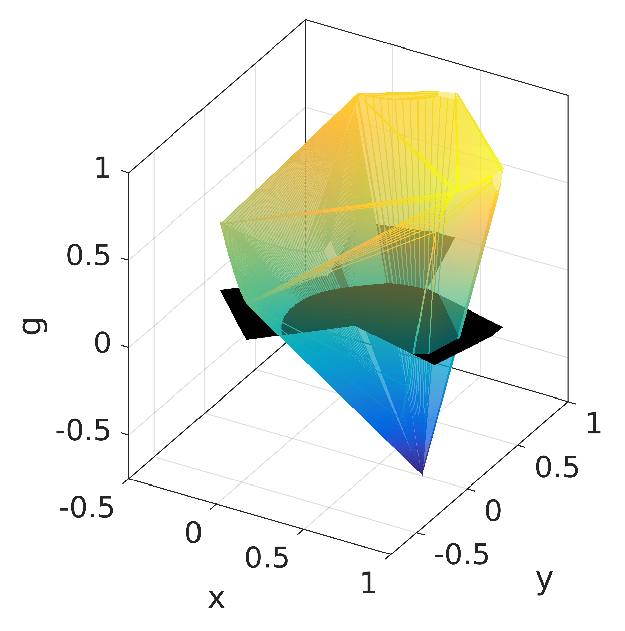
\includegraphics[width=1\linewidth]{fig/moment_hull_3}
    \caption{}
  \end{subfigure}
  \begin{subfigure}[b]{0.24\textwidth}
    \centering
    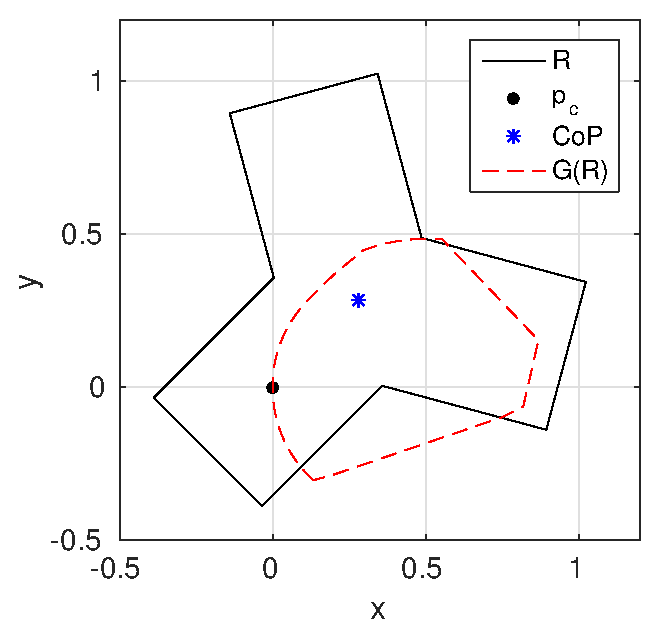
\includegraphics[width=1\linewidth]{fig/CoP_boundary}
    \caption{}
  \end{subfigure}
  \caption{Example moment envelope for a 2D tetrapod with rotation center $x_{\text{IC}} = 0.75$. (a) Support region $R$. (b) Normalized-moment surface $g(R)$. (c) Convex moment envelope $G(R)$. (d) Intersection of the moment envelope and the $xy$-plane. The intersection bounds the set of feasible centers of pressure with zero moment.}
  \label{fig:moment-envelope}
\end{figure*}

The frictional force and moment equations are
\begin{align}
  \mathbf{f}_f &= -\mu\,\sign(\dot{\theta})\,\mathbf{\hat{k}}\,\times\int_{R}\frac{\mathbf{r}-\mathbf{r_{\text{IC}}}}{\lVert \mathbf{r}-\mathbf{r_{\text{IC}}} \rVert} p(\mathbf{r}) dA \\
  \mathbf{m}_f &= -\mu\,\sign(\dot{\theta}) \int_{R}\mathbf{r}\cdot\frac{\mathbf{r}-\mathbf{r_{\text{IC}}}}{\lVert \mathbf{r}-\mathbf{r_{\text{IC}}} \rVert} p(\mathbf{r}) dA
\end{align}

Let $f_0 = \int_{R}p(\mathbf{r})dA$ be the total pressure. 
Leave $r_{\text{IC}}$ fixed.
We define the functions
\begin{align}
\mathbf{f}(\mathbf{r}) &= -\mu\,\sign(\dot{\theta})f_0\,\mathbf{\hat{k}}\,\times\frac{\mathbf{r}-\mathbf{r_{\text{IC}}}}{\lVert \mathbf{r}-\mathbf{r_{\text{IC}}} \rVert}\\
g(\mathbf{r}) &= -\mu\,\sign(\dot{\theta})f_0\,\mathbf{r}\cdot\frac{\mathbf{r}-\mathbf{r_{\text{IC}}}}{\lVert \mathbf{r}-\mathbf{r_{\text{IC}}} \rVert}
\end{align}
which are the frictional force and the frictional torque, respectively, that would result from a unit normalized pressure at $\mathbf{r}$.

Convex hull/envelope.

\section{Methods}

\subsection{Exact Angular Velocities Bounds}

\begin{proposition}
  The constrained frictional dissipation equation
  $\mathrm{D}_{\mathcal{C}}(\mathbf{v}^+)$ has a unique minimizer for
  pressure distributions with some support force off of the
  $x$-axis. When otherwise, the equation admits an interval of minima.
\end{proposition}

\begin{proof}
  The work of \cite{Mason1982} was the first to prove the above
  observation for finite pressure distributions. For the case of
  infinite (discrete) pressure distributions, we can appeal to the
  convexity properties of $\lVert A(\mathbf{x})\mathbf{v}^+ \rVert$.

  Minkowski's inequality gives
  $\lVert x + y \rVert \leq \lVert x \rVert + \lVert y \rVert$ with
  equality if and only if $x$ and $y$ are positively linearly
  dependent. For two generalized velocities
  $\mathbf{v}^+_1,\mathbf{v}^+_2\in \mathcal{C}$, the resulting body
  point velocities are linearly dependent if and only if the
  determinant
  \begin{align}
    \det A(\mathbf{x})
      \begin{bmatrix*}
        \mathbf{v}^+_1 & \mathbf{v}^+_2
      \end{bmatrix*}
    &= \det
     \begin{bmatrix*}
       -x_2\omega_1 & -x_2\omega_2 \\
       1 + x_1\omega_1 & 1 + x_1\omega_2 
     \end{bmatrix*}\\
    &= -x_2(\omega_1 - \omega_2)
  \end{align}
  is zero. We immediately see that
  $\lVert A(\mathbf{x})\mathbf{v}^+ \rVert$ is strictly convex
  relative to $\mathcal{C}$ if and only if the body point $\mathbf{x}$
  lies off of the $x$-axis. The proposition follows from the fact that
  the positive sum of convex functions and a strictly convex function
  is strictly convex.
\end{proof}

An object whose contact region is two discrete points, e.g. a spoon,
can have multiple minimizing angular velocities when aligned with the
$x$-axis.

\begin{proposition}
  Suppose $P(u) := \argmin_x f(x,u)$ with
  $f:\mathcal{X}\times\mathcal{U}\rightarrow\mathbb{R}$ continuous and
  level-set bounded. Then the set-valued mapping $P(u)$ is outer
  semi-continuous and locally bounded.
\end{proposition}

\begin{proof}
  Proposition adapted from Corollary 7.42 in \cite{Rockafellar}.
\end{proof}

\begin{theorem}
  For pulling of a planar rigid body with known center of pressure,
  the set of all feasible angular velocities is connected.
\end{theorem}

\begin{proof}
  Let us assume that the contact point moves with velocity
  $\mathbf{v}_c = [0,1]^T$. Then the generalized velocity of the
  pulled body is of the form $\mathbf{v}^+ = [0, 1, \omega]^T$. We
  want to show that the set of feasible angular velocities is a
  connected set.

  First, we argue that the frictional dissipation equation
  $\mathrm{D}(\mathbf{v}^+) = \mu\int_R\lVert
  A(\mathbf{r})\mathbf{v}^+ \rVert p(\mathbf{r})dA$
  has a unique minimum. 

  For a given body point $\mathbf{x}$, the matrix $A(\mathbf{x})$ has
  a null space spanned by $[x_2,-x_1,1]^T$. 
  \begin{equation}
    A(\mathbf{x})\mathbf{v}^+ = 
    \begin{bmatrix*}[r]
      1 & 0 & -x_2\\
      0 & 1 & x_1\\
    \end{bmatrix*} 
    \begin{bmatrix*}
      0\\ 1 \\ \omega
    \end{bmatrix*}
     = 
     \begin{bmatrix*}
       -x_2\omega \\
       1 + x_1\omega
     \end{bmatrix*}
  \end{equation}

  \begin{center}
    \bgroup
    \def\arraystretch{1.5}%  1 is the default, change whatever you need
    \begin{tabular}{r l c r}
      $\mathcal{N}(A(\mathbf{x}))$ = &$[\;x_2$ & $-x_1$ & $1\;]^T$ \\
      $\mathbf{v}^+$ = &$[\;0$ & $1$ & $\omega\;]^T$ \\
    \end{tabular}
    \egroup
  \end{center}

  Let $v^+$ be the generalized velocity. The rotation center that
  generates zero moment is the solution to 
  \begin{equation}
    \int_R\lVert A(x)v^+ \rVert d\mu(x)
  \end{equation}
  subject to 

  The image of a connected set by an outer-semicontinuous set-valued
  mapping whose values are nonempty and connected is connected
  \cite{hiriart1985images}.
\end{proof}

\begin{algorithm}
\caption{Exact Angular Velocity Bounds}\label{euclid}
\begin{algorithmic}[1]
\Procedure{Find Extrema}{$R$, $x_0$, $y_0$}
\State $\textit{stringlen} \gets \text{length of }\textit{string}$
\State $i \gets \textit{patlen}$
\BState \emph{top}:
\If {$i > \textit{stringlen}$} \Return false
\EndIf
\State $j \gets \textit{patlen}$
\BState \emph{loop}:
\If {$\textit{string}(i) = \textit{path}(j)$}
\State $j \gets j-1$.
\State $i \gets i-1$.
\State \textbf{goto} \emph{loop}.
\State \textbf{close};
\EndIf
\State $i \gets i+\max(\textit{delta}_1(\textit{string}(i)),\textit{delta}_2(j))$.
\State \textbf{goto} \emph{top}.
\EndProcedure
\end{algorithmic}
\end{algorithm}

\bibliographystyle{plainnat}
\bibliography{references}

\end{document}
